\chapter{Konfigurieren des TransistorTesters}
\label{sec:config}
Die ganze Software des TransistorTesters ist im Quellcode verfügbar.
Die Übersetzung der Module wird mit einer Makefile gesteuert. Die Entwicklung wurde
auf einem Ubuntu Linux mit den GNU-Werkzeugen (GNU toolchain, gcc version 4.5.3) durchgeführt.
Es sollte möglich sein, ohne Schwierigkeiten andere Linux-Betriebssysteme zu benutzen.
Um die übersetzen Daten in den Flash-Speicher oder den EEPROM-Speicher zu laden, wird das
Programm avrdude \cite{avrdude} (Version 5.11svn) von der Makefile benutzt, wenn man ,,make upload'' aufruft.
Das Programm avrdude ist für Linux und Windows verfügbar.
Der GNU C-Kompiler wird auch von der AVR-studio-Software unter Windows oder von
der WinAVR \cite{winavr1},\cite{winavr2} Software benutzt.
Sie können die Programmdaten (.hex und .eep) auch mit anderen Programmen in den ATmega laden,
aber nur meine Makefile-Version stellt sicher, dass die richtigen Daten in den gewählten Prozessor gelangen.
Avrdude lädt Daten nur in den ATmega, wenn die Signaturbytes des angeschlossenen ATmega gleich mit dem ausgewählten sind.
Wenn Sie die Makefile ändern, wird die Software komplett neu übersetzt, wenn man ,,make'' oder
,,make upload'' aufruft.
Die Software, die für einen ATmega8 übersetzt wurde, läuft nicht auf einem ATmega168.
Die Software, die für einen ATmega328 übersetzt wurde, läuft nicht auf einem ATmega168.
Eine Ausnahme bildet Software, die für einen ATmega168 übersetzt wurde. Diese Programmdateien
sind auch für einen ATmega328 brauchbar.
Seien Sie vorsichtig, wenn Sie nicht das mitgelieferte Makefile benutzen.

Mit den entsprechenden Optionen ist die Software auch auf dem unveränderten Hardware-Entwurf von
Markus F. lauffähig (PARTNO=m8 , {\bf keine} NO\_AREF\_CAP und {\bf keine} PULLUP\_DISABLE Option).
Die Taktrate kann mit den fuses auch auf 8MHz gestellt werden, dazu ist kein Quarz erforderlich!


Die folgenden Optionen der Makefile sind verfügbar, um die Software für den Tester zu konfigurieren:

\begin{description}
  \item[PARTNO] beschreibt den Ziel-Prozessor:\\
         m8 = ATmega8\\
         m168 or m168p = ATmega168\\
         m328 or m328p = ATmega328\\
    Beispiel: PARTNO = m168
  \item[UI\_LANGUAGE] gibt die Sprache für den Tester an:\\
    LANG\_BRASIL, LANG\_CZECH, LANG\_DUTCH, LANG\_ENGLISH, LANG\_GERMAN, \\
    LANG\_HUNGARIAN, LANG\_ITALIAN, LANG\_LITHUANIAN, LANG\_POLISH, \\
    LANG\_RUSSIAN, LANG\_SLOVAK, LANG\_SLOVENE, Lang\_SPANISH, und \\
    LANG\_UKRAINIAN sind derzeit verfügbar.
 Für die russische und ukrainische Sprache ist ein LCD mit kyrillischem Zeichensatz erforderlich.\\
    Beispiel: UI\_LANGUAGE = LANG\_ENGLISH
  \item[LCD\_CYRILLIC] wird nur gebraucht, wenn man ein LC-Display mit kyrillischem Zeichensatz benutzt.
Die Zeichen \(\mu\) und \(\Omega\) sind im kyrillischen Zeichensatz nicht enthalten.
Wenn Sie diese Option angeben, werden beide Zeichen von der Software in das LCD geladen.\\
Beispiel: CFLAGS += -DLCD\_CYRILLIC
  \item[LCD\_DOGM] muss angegeben werden, wenn ein LCD mit ST7036-Controller (Typ DOG-M) zur Anzeige verwendet wird.
Der LCD-Kontrast wird dann mit Software-Befehlen eingestellt.
Beispiel: CFLAGS += -DLCD\_DOGM
  \item[FOUR\_LINE\_LCD] kann bei einem 4x20-Zeichen-Display verwendet werden, um den Platz auf dem Display
besser auszunutzen. Zusätzliche Parameter, welche sonst nur kurz in Zeile 2 angezeigt werden, werden dann in
den Zeilen 3 und 4 angezeigt.\\
Beispiel: CFLAGS += -DFOUR\_LINE\_LCD
  \item[WITH\_LCD\_ST7665] Diese Option muss verwendet werden, wenn ein 128x64 Pixel LCD mit serieller
Schnittstelle angeschlossen ist. Für diesen Displaytyp müssen weitere Optionen gesetzt werden, die im Folgenden
beschrieben werden.
Anstelle des ST7565-Controllers kann auch der ähnliche SSD1306-Controller konfiguriert werden.
Dafür muss diese Option auf 1306 gesetzt werden.
Auch ein Display mit ST7920 oder ST7108 Controller kann angeschlossen werden. Für den ST7108 Controller muß ein
zusätzlicher Seriell-Parallel Wandler (74HCT164) verwendet werden.\\
Beispiel: WITH\_LCD\_ST7565 = 1 
 \item[LCD\_INTERFACE\_MODE] Beim SSD1306-Controller kann anstelle des Standard-SPI (4-Wire) Interface auch das
I\textsuperscript{2}C-Interface benutzt werden. Dafür muss diese Option auf 2 gesetzt werden.
Für den ST7920 Controller kann ein spezieller serieller Anschluß mit dem Setzen dieser Option auf 5
unterstützt werden.
Wenn nur eine Anschlußmöglichkeit vorgesehen ist, braucht die Konstante LCD\_INTERFACE\_MODE nicht gesetzt werden.
Der Übersicht wegen sind hier alle bisher möglichen Kennziffern aufgeführt: \\

\begin{table}[H]
  \begin{center}
    \begin{tabular}{| c | c |}
    \hline
 Kennung &  Typ der Schnittstelle \\
    \hline
    \hline
  1   & 4-Bit parallel      \\
    \hline
  2   & I\textsuperscript{2}C-Schnittstelle      \\
    \hline
  4   & 4-Bit SPI Schnittstelle      \\
    \hline
  5   & serielle Schnittstelle für ST7920      \\
    \hline
  6   & serielle Schnittstelle für ST7108 mit 74HCT164  \\
    \hline
    \end{tabular}
  \end{center}
  \caption{Kennziffern für die Art der Schnittstelle}
\end{table}

Beispiel: CFLAGS += -DLCD\_INTERFACE\_MODE=2
 \item[LCD\_I2C\_ADDR] Die I\textsuperscript{2}C-Adresse des SSD1306-Controllers kann durch Vorbesetzen der Adresse LCD\_I2C\_ADDR
auf 0x3D geändert werden.\\
Beispiel: CFLAGS += -DLCD\_I2C\_ADDR=0x3d
  \item[LCD\_ST7565\_RESISTOR\_RATIO] Mit dieser Option wird das Widerstands-Teilerverhältnis für den
Spannungsregler des ST7565-Controllers eingestellt. Brauchbare Werte liegen im Allgemeinen zwischen 4 und 7.
Einstellbar sind Werte zwischen 0 und 7.\\
Beispiel: LCD\_ST7564\_RESISTOR\_RATIO = 4
  \item[LCD\_ST7565\_H\_FLIP] Mit dieser Option kann die Anzeige horizontal umgedreht werden.\\
Beispiel: CFLAGS += LCD\_ST7565\_H\_FLIP = 1
  \item[LCD\_ST7565\_H\_OFFSET] Diese Option kann den für die Ausgabe benutzten Speicher an das Anzeigefenster des
 Displays anpassen. Der Controller benutzt mehr horizontale Pixel (132) als angezeigt (128) werden.
 Je nach Lage des Anzeigefenster muss der Offset bei gedrehter oder normaler horizontaler Anzeigerichtung
 berücksichtigt werden.
 Ein Wert von 0, 2 oder 4 kann je nach verwendetem Display-Modul für eine korrekte Darstellung notwendig sein.\\
Beispiel: CFLAGS += LCD\_ST7565\_H\_OFFSET = 4
  \item[LCD\_ST7565\_V\_FLIP] Mit dieser Option kann die Anzeige vertikal umgedreht werden.\\
Beispiel: CFLAGS += LCD\_ST7565\_V\_FLIP = 1
  \item[FONT\_8X16] Für den ST7565 controller sollte ein Fonts ausgewählt werden.
Auswählbar  sind FONT\_6X8, FONT\_8X8, FONT\_8X12, FONT\_8X14 FONT\_8X15, FONT\_8X16 und FONT\_8X16thin.
Derzeit ist der Font 8x12 nicht fertiggestellt.
Die Fontgröße 8X16 ist die effizienteste Wahl für das graphische 128x64-LCD.\\
Beispiel: CFLAGS += FONT\_8X16
  \item[STRIP\_GRID\_BOARD] Diese Option passt die Software an eine andere Pinbelegung von Port~D für Streifenleiterplatinen an.
Die Einzelheiten findet man im Hardwarekapitel \ref{sec:hardware}.
Beispiel: CFLAGS += -DSTRIP\_GRID\_BOARD
  \item[WITH\_MENU] aktiviert eine Menüfunktion für einen ATmega328. Man kann einige Zusatzfunktionen über ein
Auswahlmenü benutzen, welches man über einen langen Tastendruck (\textgreater~0,5~s) erreichen kann.
Wenn die Menüfunktion eingeschaltet ist, wird beim automatischen Selbsttest-Start mit kurzgeschlossenen Testpins
 nur der Kalibrationsteil des Selbsttests ausgeführt.
Die Tests T1-T7 werden nur beim Selbsttest ausgeführt, der als Menüfunktion ausgewählt werden kann.\\
Beispiel: CFLAGS += -DWITH\_MENU
  \item[WITH\_ROTARY\_SWITCH] Die Menüfunktion kann leicher bedient werden, wenn ein Impulsdrehgeber als Erweiterung
benutzt wird.
Für die Details der notwendigen Erweiterung sehen Sie bitte die Beschreibung~\ref{fig:RotExt} im Hardwarekapitel.
Wenn der Impulsdrehgeber die gleiche Anzahl von Raststellungen wie Impulse für jede Umdrehung hat,
muss die Option WITH\_ROTARY\_SWITCH auf 2 gesetzt werden.
Wenn der Impulsdrehgeber doppelt so viele Raststellungen hat, muss die Option WITH\_ROTARY\_SWITCH auf 1 gesetzt werden.
Das Setzen der Option \_WITH\_ROTARY\_SWITCH auf 5 wählt die höchste Auflösung für den Impulsdrehgeber.
Jeder Zyklus der beiden Schalter-Zustände wird als 4 gezählt. Normalerweise ist diese Einstellung nur für
Impulsdrehgeber ohne Raststellung sinnvoll.
Ein Setzen der Option WITH\_ROTARY\_SWITCH auf 4 ist notwendig für die korrekte Behandlung von zwei separaten
Rauf (Up) und Runter (Down) Tastern, die anstelle der beiden Schalter eines Impulsdrehgebers eingebaut sind.
Verwenden Sie nicht die Einstellung 4 mit normalen Impulsdrehgebern!\\
Beispiel: CFLAGS += -DWITH\_ROTARY\_SWITCH=1
  \item[CHANGE\_ROTARY\_DIRECTION] Man kann die erkannte Drehrichtung des Impulsdrehgebers durch Vertauschen
der beiden Schalter-Signale oder durch Setzen dieser Option ändern.
Beispiel: CFLAGS += -DCHANGE\_ROTARY\_DIRECTION
 \item[WITH\_SELFTEST] Wenn Sie diese Option angeben, baut die Software eine Selbsttest-Funktion ein, die gestartet wird
wenn Sie alle drei Prüfspitzen verbinden und eine Messung starten.\\
Beispiel: CFLAGS += -DWITH\_SELFTEST
  \item[NO\_COMMON\_COLLECTOR\_HFE] verhindert die hFE-Messung von Transistoren in der Kollektorschaltung.
So können Sie Speicher sparen, um die erweiterten Selbsttest-Routinen T1 bis T7 für den ATmega168-Prozessor zu ermöglichen.
Standardmäßig sind beide Schaltungen für die hFE-Messung eingeschaltet,
aber dann ist kein Platz im Programmspeicher des ATmega168 für die erweiterten Selbsttests.\\
Beispiel: CFLAGS += -DNO\_COMMON\_COLLECTOR\_HFE
  \item[NO\_COMMON\_EMITTER\_HFE] schaltet die hFE-Messung von Transistoren in Emitterschaltung ab.
So können Sie Speicher sparen, um die erweiterten Selbsttest-Routinen T1 bis T7 für den ATmega168-Prozessor zu ermöglichen.
Standardmäßig sind beide Schaltungen für die hFE-Messung eingeschaltet,
aber dann ist kein Platz im Programmspeicher des ATmega168 für die erweiterten Selbsttests.\\
Beispiel: CFLAGS += -DNO\_COMMON\_EMITTER\_HFE
  \item[NO\_TEST\_T1\_T7] Diese Option verhindert die Ausführung der Selbsttest Teile T1 bis T7.
Diese Tests sind nützlich um Fehler in der Schaltung wie falsche Messwiderstände oder Isolationsprobleme zu finden.
Wenn Ihre Schaltung fehlerfrei ist, können Sie die Selbsttest-Teile T1 bis T7 durch das Setzen dieser Option weglassen, um eine
schnellere Kalibration zu erreichen.
Bei eingeschalteter Menüfunktion werden die Selbsttest-Teile T1 bis T7 nur bei Aufruf der Menüfunktion ,,Selbsttest'' ausgeführt.
Der ATmega168-Prozessor benutzt die Selbsttest Teile T1 bis T7 nicht, wenn beide Messmethoden für die hFE-Bestimmung benutzt werden.\\
Beispiel: CFLAGS += -DNO\_TEST\_T1\_T7
  \item[AUTO\_CAL] Der Nullabgleich für die Kondensatormessung wird beim
Selbsttest zusätzlich ins EEPROM geschrieben und ist damit für die weiteren Messungen abgeglichen.
Wenn nach dem Nullabgleich der Kondensatormessung ein Kondensator mit einer Kapazität zwischen \(100 nF\) und \(20 \mu F\) an Pin~1 und Pin~3 
angeschlossen wird, wird auch der Offset des analogen Komparators und die Skalierung für die AUTOSCALE\_ADC
Umschaltung auf die interne Spannungsreferenz ermittelt und ins EEPROM geschrieben.
Die Port-Ausgangswiderstände werden zu Beginn jeder Messung neu bestimmt. \\
Beispiel: CFLAGS += -DAUTO\_CAL
  \item[FREQUENCY\_50HZ] Zum Ende des Selbsttests wird bis zu einer Minute lang ein 50Hz-Signal auf Port 2 und Port 3 erzeugt.\\
Beispiel: CFLAGS += -DFREQUENCY\_50HZ
  \item[CAP\_EMPTY\_LEVEL] Diese Option legt die Spannung (mV) für einen entladenen Kondensator fest.
Der Wert kann höher als 3mV gesetzt werden, wenn die Entladung nicht zum Ende kommt. In diesen Fall meldet der Tester nach längerer Zeit ,,Cell!''.\\
Beispiel: CFLAGS += -DCAP\_EMPTY\_LEVEL=3
  \item[WITH\_AUTO\_REF] Mit dieser Option wird die Referenzspannung gemessen, um den aktuellen Faktor für die Kapazitätsmessung 
von kleineren Kapazitäten (unter \(40\mu F\)) zu ermitteln.\\
Beispiel: CFLAGS += -DWITH\_AUTO\_REF
  \item[REF\_C\_KORR] gibt einen Offset für die gelesene Referenz-Spannung in mV-Einheiten an.
Das kann benutzt werden, um die Kapazitätsmessung kleiner Kondensatoren abzugleichen.
Wenn zusätzlich die AUTO\_CAL-Option gewählt wurde, ist diese Angabe nur ein zusätzlicher Offset für
den gefundenen Komparator-Offset.
Ein Wert von 10 ergibt etwa 1~Prozent kleinere Messergebnisse.\\
Beispiel: CFLAGS += -DREF\_C\_KORR=14
  \item[REF\_L\_KORR] gibt einen zusätzlichen Offset für die Referenz-Spannung für die Induktivitätsmessung
in mV-Einheiten an. Der REF\_C\_KORR-Offset beziehungsweise der gefundene Offset bei der Kalibration
wird bei der Induktivitätsmessung ebenfalls berücksichtigt.\\
Der REF\_L\_KORR Wert wird für die Messungen ohne \(680 \Omega\) Widerstand subtrahiert, bei Messungen mit einem
\(680 \Omega\) Widerstand wird der Wert addiert.
Ein Wert von 10 führt zu einer Änderung des Ergebnisses um 1 Prozent.\\
Beispiel: CFLAGS += -DREF\_L\_KORR=40
  \item[C\_H\_KORR] gibt eine Korrektur der Messergebnisse für grosse Kondensatoren an.
Eine Eingabe von 10 führt zu 1~Prozent kleineren Messergebnissen.\\
Beispiel: CFLAGS += -DC\_H\_KORR=10
  \item[WITH\_UART] benutzt den Pin PC3 zur Ausgabe der seriellen Texte (V24). Wenn die Option nicht
benutzt wird, kann der PC3 Pin zum Anschluss einer externen Spannung mit einem 10:1-Widerstandsteiler benutzt
werden. Damit können beispielsweise Zenerdioden mit höherer Durchbruchspannung getestet werden.
Diese Messung wird so lange mit etwa 3 Messungen pro Sekunde wiederholt, solange der Starttaster gedrückt bleibt.\\
Beispiel: CFLAGS += -DWITH\_UART
  \item[TQFP\_ADC6] Die Option TQFP\_ADC6 benutzt anstelle des PC3-Pins (ADC3) den zusätzlichen ADC-Eingang ADC6
des ATmegas im TQFP-Gehäuse oder QFN-Gehäuse.
Dadurch kann dieser Eingang unabhängig von der seriellen Ausgabe auf dem PC3 Pin genutzt werden. Dieser Pin wird
dann für die Zenerdioden-Messung und für die Messung einer externen Spannung über den Dialog des ATmega328 genutzt.\\
Beispiel: CFLAGS += -DTQFP\_ADC6
  \item[TQFP\_ADC7] Die Option TQFP\_ADC7 benutzt anstelle des PC3-Pins (ADC3) den zusätzlichen ADC-Eingang ADC7
des ATmegas im TQFP-Gehäuse und QFN-Gehäuse.
Dadurch kann dieser Pin unabhängig von der seriellen Ausgabe auf den PC3 Pin genutzt werden. Wenn diese Option 
ohne die Option TQFP\_ADC6 genutzt wird, erfolgt sowohl die Zenerdioden-Messung als auch die Messung einer externen
Spannung über den Dialog des ATmega328 genutzt. Wenn die Option zusätzlich zur TQFP\_ADC6-Option gesetzt wird,
erfolgt die Zenerdioden-Messung mit dem ADC6-Pin und bei der über den Dialog wählbaren Spannungsmessung werden
beide Eingänge gemessen. Beide Pinne sollten dann an einen 10:1-Spannungsteiler angeschlossen sein.\\
Beispiel: CFLAGS += -DTQFP\_ADC7
  \item[WITH\_VEXT] ermöglicht die Messung einer externen Spannung über einen 10:1-Spannungsteiler.
Für den ATmega168 oder ATmega328 wird normalerweise der PC3-Pin benutzt, wenn keine Option TQFP\_ADC6 oder
TQFP\_ADC7 gesetzt ist. Dann ist diese Option aber nur möglich, wenn die WITH\_UART Option nicht gesetzt ist.\\
Beispiel: CFLAGS += -DWITH\_VEXT 
  \item[AUTOSCALE\_ADC] schaltet die automatische Bereichswahl des ADC (entweder VCC oder interne Referenz) ein.
Die interne Referenz hat 2,56V für den ATmega8 und 1,1V für die anderen Prozessoren.\\
Beispiel: CFLAGS += -DAUTOSCALE\_ADC
  \item[ESR\_ZERO] gibt einen Nullwert für die ESR-Messung von Kondensatoren vor.
Der vorgegebene Nullwert wird durch die beim Selbsttest ermittelten Nullwerte für alle drei Pinkombinationen ersetzt.
 Diese Nullwerte werden von den ermittelten Messwerten abgezogen.
Beispiel: CFLAGS += -DESR\_ZERO=29
  \item[NO\_AREF\_CAP] teilt der Software mit, dass Sie keinen Kondensator am AREF Pin (Pin 21) angeschlossen haben.
Dies ermöglicht kürzere Wartezeiten für die AUTOSCALE\_ADC Umschaltung des ADC.
Ein 1nF Kondensator wurde in diesem Modus ohne Fehler getestet.
Die Abbildungen~\ref{pic:aref1} und \ref{pic:aref5} zeigen die Schaltzeiten mit einem 1nF Kondensator.
Wie Sie sehen können ist das Schalten von 5V auf 1,1V viel langsamer als das Zurückschalten auf 5V.
Wenn Sie noch einen \(100 nF\) installiert haben, ist die Schaltzeit etwa Faktor 100 länger!\\
Beispiel: CFLAGS += -DNO\_AREF\_CAP

\end{description}

\begin{figure}[H]
  \begin{subfigure}[b]{8.6cm}
    \centering
    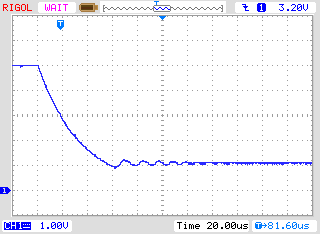
\includegraphics[width=8.3cm]{../PNG/AREF2_1V.png}
    \caption{from 5V to 1.1V }
    \label{pic:aref1}
  \end{subfigure}
  ~
  \begin{subfigure}[b]{8.6cm}
    \centering
    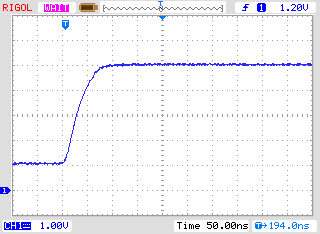
\includegraphics[width=8.3cm]{../PNG/AREF2VCC.png}
    \caption{from 1.1V to 5V}
    \label{pic:aref5}
  \end{subfigure}
  \caption{Umschalten von AREF mit einem \(1nF\) Kondensator}
\end{figure}

\begin{description}
  \item[REF\_R\_KORR] gibt einen Offset für die interne Referenz-Spannung in mV-Einheiten an.
Mit diesem Offset kann eine Differenz bei der Umschaltung der Referenzspannung für die Widerstandsmessung abgeglichen werden.
Wenn die AUTO\_CAL-Option gewählt wurde, ist dieser Wert nur ein Offset zu der gefundenen Spannungs-Differenz in der
AUTO\_CAL Funktion.\\
Beispiel: CFLAGS += -DREF\_R\_KORR=10
  \item[OP\_MHZ] gibt der Software an, mit welcher Taktfrequenz in MHz der Tester arbeiten wird.
Die Software ist nur mit 1MHz, 8MHz und zusätzlich auch 16MHz getestet. Der Betrieb mit 8MHz wird wegen der besseren Auflösung der
Kondensator- und Spulen-Messung empfohlen.\\
Beispiel: OP\_MHZ = 8
  \item[RESTART\_DELAY\_TICS] muss auf 6 gesetzt werden, wenn der ATmega168 oder ATmega328 ohne Quarz mit dem
RC-Generator betrieben wird. Wenn dieser Wert nicht vorbesetzt wird, wählt die Software die 16384 Takte Startverzögerung für
den Quarzbetrieb.\\
Beispiel: CFLAGS += -DRESTART\_DELAY\_TICS = 6
  \item[USE\_EEPROM] gibt an, ob feste Texte und Tabellen im EEPROM-Speicher abgelegt werden sollen.
Anderenfalls wird der Programmspeicher (Flash) benutzt.
Es wird empfohlen, den EEPROM-Speicher zu benutzen (Option gesetzt).\\
Beispiel: CFLAGS += -DUSE\_EEPROM
  \item[EBC\_STYLE] gibt an, dass die Ausgabe der Transistor-Pinbelegung im Format ,,EBC=...'' bzw. ,,GDS=...'' erfolgen soll.
Diese Darstellungsweise spart Programmplatz. Ohne diese Option wird die Belegung im Format ,,123=...'' angezeigt, wobei
jeder Punkt ein E (Emitter), B (Basis) oder K (Kollektor) sein kann.
Bei FETs kann jeder Punkt entsprechend ein G (Gate), D (Drain) oder S (Source) sein.
Wenn die Reihenfolge der Testpins nicht 1,2 und 3 in Leserichtung ist, kann die Reihenfolge mit der Option EBC\_STYLE=321 
umgedreht werden. Dann wird die Pinbelegung in der Form ,,321=...'', was der gewohnten Leserichtung von links nach rechts
entgegen kommt.\\
Beispiel: CFLAGS += EBC\_STYLE
  \item[NO\_NANO] gibt an, dass der Dezimalpräfix Nano nicht zur Darstellung von Messergebnissen benutzt werden soll.
So werden Kapazitätswerte in \(\mu F\) statt in \(nF\) angegeben.\\
Beispiel: CFLAGS += NO\_NANO
  \item[PULLUP\_DISABLE] gibt an, dass man die internen ,,Pull-Up''-Widerstände nicht benötigt.
 Sie müssen einen externen ,,Pull-Up'' Widerstand an Pin 13 (PD7) und VCC angeschlossen haben, um diese
Option benutzen zu können.
Mit dieser Option wird ein möglicher Einfluss der ,,Pull-Up'' Widerstände auf die Mess-Ports (Port B und Port C) verhindert.\\
Beispiel: CFLAGS += -DPULLUP\_DISABLE
  \item[ANZ\_MESS] diese Option gibt an, wie oft der ADC-Wert eingelesen und addiert werden soll.
Sie können einen Wert zwischen 5 und 200 wählen um einen Mittelwert für eine ADC-Messung zu bilden.
Höhere Werte ergeben eine bessere Genauigkeit, aber brauchen längere Messzeit.
Eine ADC-Messung mit dem Wert 44 braucht etwa 5ms.\\
Beispiel: CFLAGS += -DANZ\_MESS=44
  \item[POWER\_OFF] Diese Option schaltet die automatische Abschaltfunktion ein.
Wenn Sie diese Option weglassen, werden die Messungen in einer Schleife endlos wiederholt, bis die Betriebsspannung 
unterbrochen wird (Ein/Aus-Schalter).
Wenn Sie einen Tester ohne die Schalttransistoren haben, können Sie diese Option weglassen.

Wenn Sie mit den eingebauten Schalttransistoren die Option POWER\_OFF weggelassen haben,
gibt es dennoch eine Möglichkeit für eine Abschaltung, wenn Sie die WITH\_MENU-Option gewählt haben.

Sie können mit der POWER\_OFF-Option auch angeben, nach wie vielen Messungen ohne gefundenes Bauteil der Tester ausschaltet.
Bei doppelt so viel aufeinanderfolgenden Messungen mit gefundenem Bauteil schaltet der Tester auch ab,
wenn nicht zwischendurch eine Messung ohne gefundenes Bauteil war.
Wenn Sie vergessen haben, ein angeschlossenes Bauteil abzuklemmen, wird so eine vollständige Batterie-Entladung
verhindert.
Bei einer Options-Angabe in der Form von CFLAGS += -DPOWER\_OFF=5 wird nach 5 aufeinanderfolgenden Messungen ohne
gefundenes Bauteil abschaltet. Aufeinanderfolgende 10 Messungen mit gefundenem Bauteil schalten ebenfalls aus.
Nur wenn die jeweilige Mess-Serie durch den anderen Typ unterbrochen wird, wird die Messung fortgesetzt.
Die Messresultate für eine Einzelmessung werden 28~Sekunden angezeigt, bei der Mehrfachmessung wird die
Anzeigezeit auf 5~Sekunden reduziert (wird in config.h gesetzt).
Wenn der Startknopf beim ersten Einschalten lange gedrückt wird, wird das Messergebnis
 auch bei der Mehrfachmessung 28~Sekunden angezeigt.
Der Maximalwert für die Wiederholungen ist 255 (CFLAGS += -DPOWER\_OFF=255).\\
Beispiel 1: CFLAGS += -DPOWER\_OFF=5 \\
Beispiel 2: CFLAGS += -DPOWER\_OFF 
  \item[BAT\_CHECK] schaltet die Batterie-Spannungsprüfung ein.
 Wenn Sie diese Option nicht angeben, wird die Versionsnummer der Software angezeigt.
Diese Option ist hilfreich um bei batteriebetriebenen Tester-Versionen an den Batteriewechsel zu erinnern.\\
Beispiel: CFLAGS += -DBAT\_CHECK
  \item[BAT\_OUT] schaltet die Batterie-Spannungsanzeige auf dem LCD ein, wenn BAT\_CHECK gewählt wurde.
 Wenn Ihre 9V-Versorgung eine Diode als Verpolungsschutz installiert hat, können Sie 
die Form BAT\_OUT=600 angeben, um die Dioden-Schwellspannung 
bei der Spannungsanzeige zu berücksichtigen.
Auch der Spannungsverlust am Transistor T3 kann so mit dieser Option berücksichtigt werden.
Die Angabe der Schwellspannung in mV beeinflusst nicht die Prüf\-span\-nungs Werte (BAT\_POOR).\\
Beispiel 1: CFLAGS += -DBAT\_OUT=300 \\
Beispiel 2: CFLAGS += -DBAT\_OUT
  \item[BAT\_POOR] setzt die Leer-Spannung für die Batteriespannungs-Prüfung auf den angegebenen Wert in Einheiten von 1mV.
Die Warn-Spannung ist 0,8V höher als die angegebene Leer-Spannung, wenn die Leer-Spannung mehr als 5,3V beträgt.
Sonst wird eine 0,4V höhere Warn-Spannung gewählt, bei unter 3,25V sogar nur eine 0,2V höhere Warn-Spannung und
bei unter 1,3V nur eine 0,1V höhere Warnspannung als die angegebene Leer-Spannung.
Das Setzen der Leer-Spannung auf Werte wie 5,4V wird für wiederaufladbare 9V Batterien nicht empfohlen,
weil das die Gefahr von Batterie-Schäden aufgrund von Tiefentladung erhöht!
Wenn Sie wiederaufladbare 9V-Batterien einsetzen, werden ,,Ready to Use''-Typen wegen der geringeren Selbstentladung empfohlen.\\
Beispiel für low-drop-Regler (5,4V): CFLAGS += -DBAT\_POOR=5400 \\
Beispiel für 7805-Regler (6,4V): CFLAGS += -DBAT\_POOR=6400
  \item[INHIBIT\_SLEEP\_MODE] sperrt die Benutzung des ,,Sleep Mode'' (Schlafzustand) des Prozessors.
Normalerweise wird von der Software für längere Pausen der Schlafzustand des Prozessors benutzt, um Strom zu sparen.
Die Benutzung dieses Schlafzustandes mit dem Wiederaufwachen spart zwar Batteriekapazität, 
stellt eine zusätzliche Anforderung für den Spannungsregler dar.\\
Beispiel: CFLAGS += -DINHIBIT\_SLEEP\_MODE
  \item[PROGRAMMER] stellt den Programmer-Typ für das avrdude Schnittstellenprogramm ein.
Eine richtige Einstellung des Programmer-Typs (und Ports) ist notwendig, wenn Sie den ,,make upload''- oder
,,make fuses''-Aufruf dieser Makefile benutzen.
Für weitere Informationen schauen Sie bitte in das Handbuch von avrdude oder in die Online-Dokumentation~\cite{avrdude}.\\
Beispiel: PROGRAMMER=avrisp2
  \item[BitClock] stellt die Bit-Taktperiode für den Programmer ein. Siehe dazu die Beschreibung des -B Parameters von avrdude.\\
Beispiel: BitClock=5.0
  \item[PORT] stellt die verwendete Schnittstelle ein, wo avrdude den Mikrocontroller (ATmega) erreichen kann.
Für weitere Informationen schauen Sie bitte ins Handbuch von avrdude.\\
Beispiel: PORT=usb

\end{description}

Zusätzliche Parameter können in den Dateien Transistortester.h und config.h gesetzt werden.
Die Datei config.h enthält globale Variablen und Tabellen, definiert die Port- / Pin-Konstellation,
die ADC-Taktfrequenz sowie die Widerstandswerte, die für die Messung benutzt werden.
Die Datei Transistortester.h enthält die globalen Variablen und Tabellen sowie die Texte für die LCD-Anzeige.
Normalerweise brauchen diese Werte nicht ohne Grund geändert werden.
